\documentclass[UTF-8, a4paper, 12pt]{ctexart}

\usepackage[left=1in,right=1in,top=1.00in,bottom=1.00in]{geometry}
\usepackage[colorlinks,linkcolor=blue,anchorcolor=blue,citecolor=green,CJKbookmarks=True]{hyperref}
\usepackage{CJK,CJKnumb}
%\usepackage{indentfirst}        % 首行缩进宏包
%\usepackage{latexsym,bm}        % 处理数学公式中和黑斜体的宏包
\usepackage{amsmath,amssymb}     % AMSLaTeX宏包 用来排出更加漂亮的公式
\usepackage{graphicx}
\usepackage{cases}
\usepackage{pifont}
\usepackage{txfonts}
\usepackage{subfigure}
\usepackage{pdfpages}
\usepackage{listings}
\usepackage{xcolor}
\usepackage[subfigure]{tocloft}     % 模板中用了subfigure,不加此选项会产生冲突

\CTEXsetup[format={\Large\bfseries}]{section}
\zihao{-4}\linespread{1.5}\selectfont
\renewcommand{\theequation}{\arabic{section}-\arabic{equation}}
\renewcommand{\thefigure}{\arabic{section}-\arabic{figure}}
%\renewcommand{\thefigure}{\thechapter-\arabic{figure}}


\renewcommand{\cftsecleader}{\cftdotfill{\cftdotsep}}
\renewcommand\contentsname{{\qquad\qquad\qquad\qquad\qquad\qquad 目\quad 录}}
\newcommand{\song}{\CJKfamily{song}}    % 宋体   (Windows自带simsun.ttf)

\title{\bfseries \Huge  基于FPGA的居家锻炼运动教学系统}
\author{胡森康,张益畅}
\date{\today}

\begin{document}
%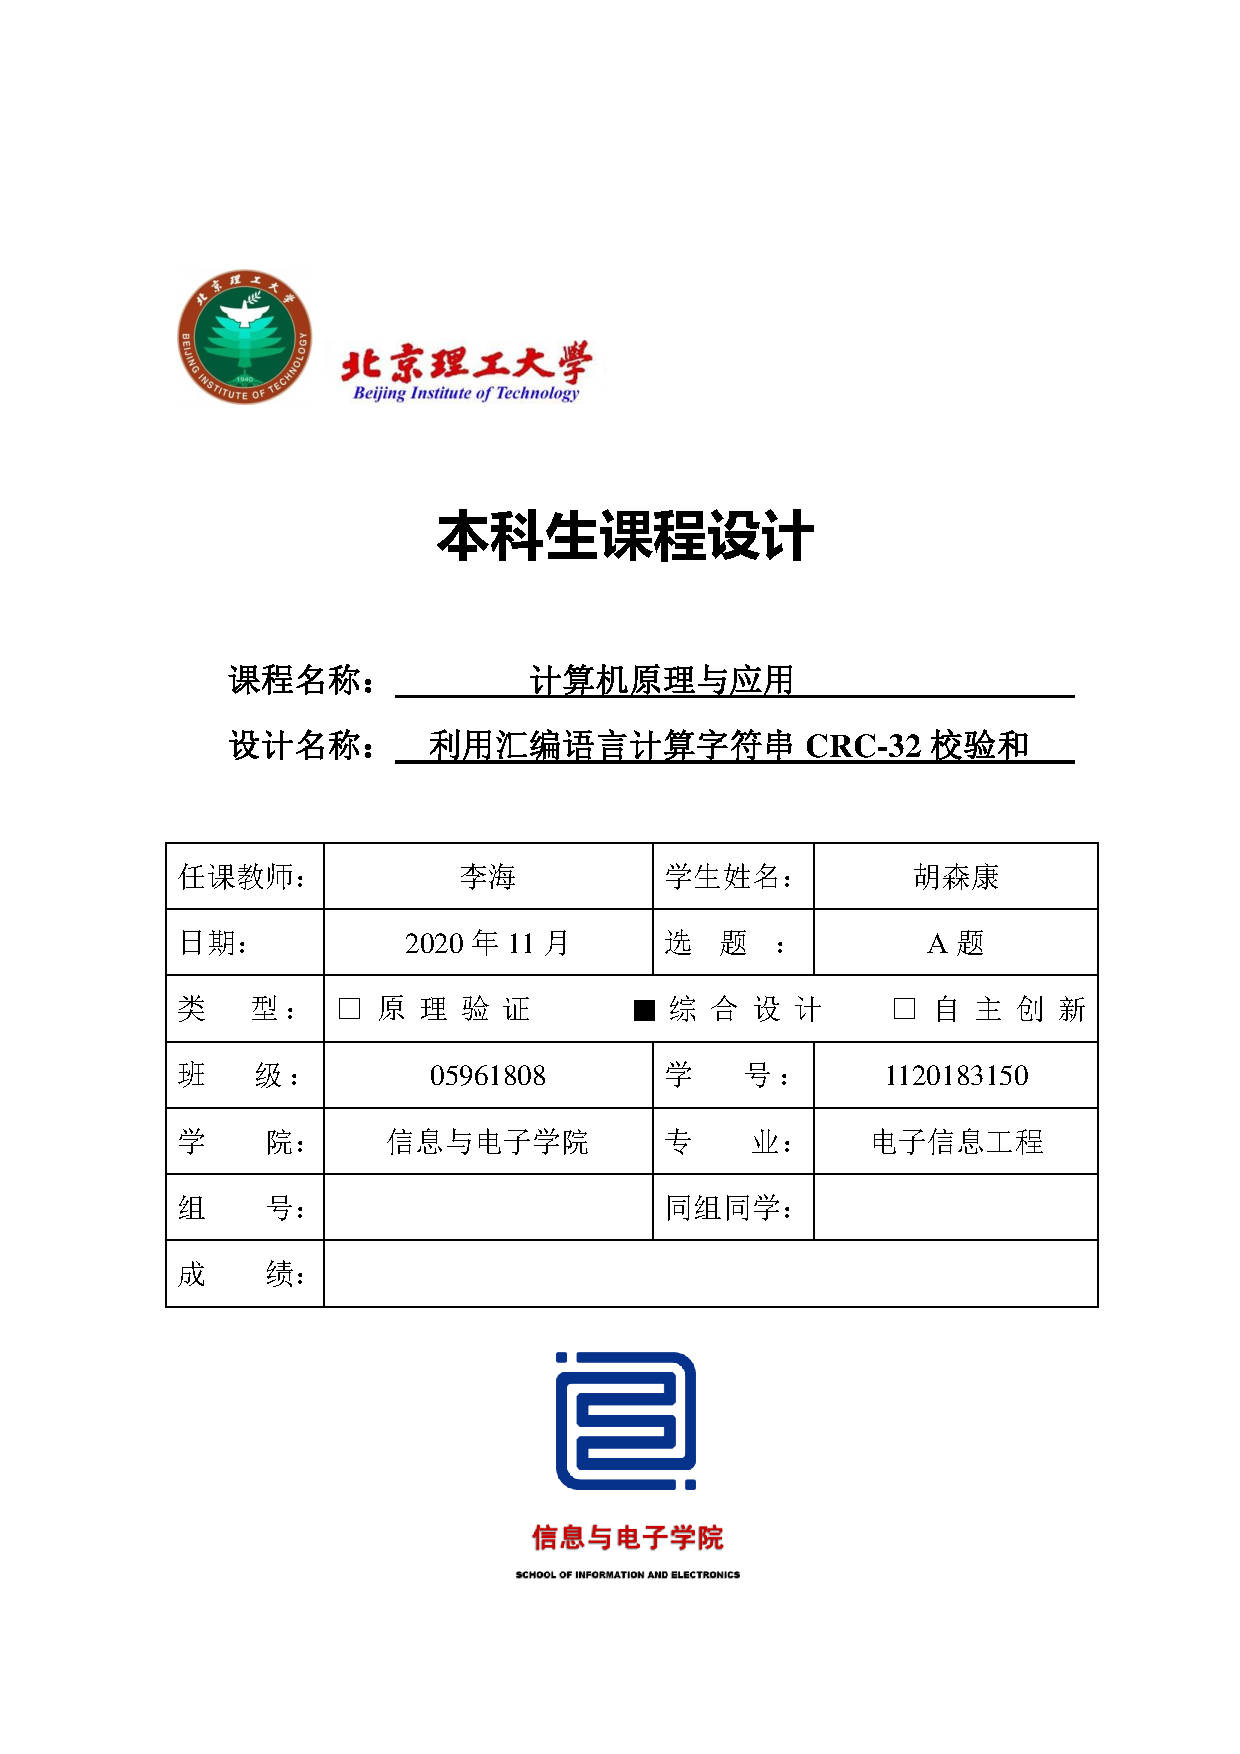
\includepdf[pages={1}]{coverpage.pdf} %% 插入pdf
\maketitle
\thispagestyle{empty}
\newpage
\thispagestyle{empty}

\tableofcontents
\newpage

\section{设计概述}
\subsection{设计目的}
2020年初,新冠肺炎疫情袭卷全球,疫情肆虐,病毒横行,国家出台一
系列防护措施保护人民群众生命安全。其中“居家令”等措施建议居民非
必要不外出,因此居民居家时间大幅度延长,户外锻炼次数大幅度减少。
基于此背景,我们希望可以开发出一种可以智能辅助人们居家锻炼如瑜
伽,体操,健身,跳舞等运动的系统,此系统用于识别人体动作,判断
动作的准确性,以此达到响应号召,足不出户,也可以锻炼身体的目的。

\subsection{应用领域}
此系统从当前全球最热点的问题,新冠肺炎疫情出发设计而成,可
应用于居民居家锻炼,此外该系统功能为识别人体动作,也可以用于
其他领域,如智能家居,交互游戏,智能人机交互,身份识别,视频监
控,健身舞蹈,视频审查,安全防控,交互娱乐,体感游戏等。

\subsection{主要技术特点}
我们设计的基于FPGA的居家锻炼运动教学系统,通过对摄像头拍
到的人体运动姿态进行识别,提取人体动作的某些特征来判断人的
姿态所蕴含的意义。将姿态与现有数据进行比对。通过图像传感采
集人体姿态,对姿态图像进行中值滤波,二值化,姿态分割,并建立
人体六星模型,进行特征提取和数据比对,最终将处理后的图像
显示在屏幕上,
并显示出识别的结果。

\subsection{关键性能指标}
关键性能指标在于如何能够准确地识别出采集到的人体姿态。
基于样本集的人体动作的识别算法,我们采用建立人体六星模
型的方法构造人体姿态的特征向量,即结合图像投影分割技术
得到六点,取质心点$(X_c,Y_c)$,矩形均分左右两部分,各取两区域内
最高最低最边点共6点$(X_i,Y_i), i=1,2,3,4,5,6$。将质心点到6个点
的欧式距离以及质心与6个点的连线与水平坐标夹角,共12个特
征作为特征向量对人体动作进行描述。

主要创新点:
\begin{enumerate}
    \item 采用图像分割投影技术,红框内得到图像即为处理后的结果。
    \item 识别算法采用多特征融合的人体行为描述算子来表征人
    体姿态特征,包括六星与质心的欧氏距离,六星角度。
\end{enumerate}

\section{系统组成及功能说明}

\subsection{整体介绍}

本系统使用了Xillinx公司的Artix-7系列的1CSG324C

首先设计如下图所示的系统框图,本次实验包括以下模块
:时钟模块、图像分辨率设置模块、DDR控制器模块、摄像
头驱动模块、图像处理模块及特征识别模块、数码管驱动模
块和LCD 顶层模块。

\begin{figure}[htbp]
    \centering
    
\includegraphics[width=15cm]{figs/f1.png}
    \caption{系统整体框图}
\end{figure}

FPGA 顶层模块($ov5640\_lcd$)例化了以下六个模块:

时钟模块($clk\_wiz\_0$)、OV5640 驱动模块($ov5640\_dri$
)、摄像头图像分辨率设置模块($picture_size$)、DDR 控
制模块($ddr3\_top$)和LCD 顶层模块($lcd\_rgb\_top$)、数
码管驱动模块和图像处理及特征识别模块(vip)。
\begin{enumerate}
    \item 时钟模块($clk\_wiz\_0$):时钟模块通过调用MMCM IP 核实现,共
输出2 个时钟,频率分别为200Mhz(DDR3 参考时钟)和50Mhz 时
钟。200Mhz 时钟作为DDR 控制模块的参考时钟,由MIG IP 核产生
的$ui\_clk$(本次设计为100Mhz)作为DDR 控制模块的驱动时钟,50
Mhz 时钟作为OV5640 驱动模块、摄像头图像分辨率设置模块和LCD
顶层模块的驱动时钟。
\item OV5640 驱动模块($ov5640\_dri$):OV5640 驱动模块负责驱动
OV5640 SCCB 接口总线,将像素时钟驱动下的传感器输出的场同
步信号、行同步信号以及8 位数据转换成DDR 读写控制模块的写使
能信号和16位写数据信号,完成对OV5640 传感器图像的采集。
\item 图像分辨率设置模块($picture\_size$):图像尺寸配置模块用于
配置摄像头输出图像尺寸的大小,此外还完成了DDR3 的读写结束
地址设置。
\item DDR 控制模块($ddr3\_top$):DDR 读写控制器模块负责驱动DDR
片外存储器,缓存图像传感器输出的图像数据。该模块将MIG IP
核复杂的读写操作封装成类似FIFO 的用户接口,非常方便用户
的使用。
\item LCD 顶层模块($lcd\_rgb\_top$):LCD 顶层模块负责
驱动LCD 屏的驱动信号的输出,同时为其他模块提供
屏体参数、场同步信号和数据请求信号。
\item 图像处理和特征提取模块($vip$):在LCD顶层
提取图像信息,并对图像进行处理和识别,并在LCD
屏中显示处理过后的图形。
\item 数码管显示模块:将识别到的结果显示在数码
管上。
\end{enumerate}













\subsection{各个模块介绍}

根据总体系统框图,给出各模块的具体设计说明。
\subsubsection{摄像头模块}
    本系统采用0V5640摄像头,
    设定为1280*800分辨率,帧率为60fps进行图像的拍摄。
    图像输出为RGB565格式,便于后续的图像处理。


\subsubsection{图像格式转换模块}
    在该模块,图像从RGB图像转换为灰度图像。
    具体做法为先从RGB565格式转换为YCbCr格式,然后只输出图像亮度信息,
    即完成了图像从彩色到灰度的转换。图像变为灰度之后,便于下一步进行处
    理提取出人体的姿态。

\subsubsection{图像处理和特征提取模块}
\begin{figure}[htbp]
    \centering
    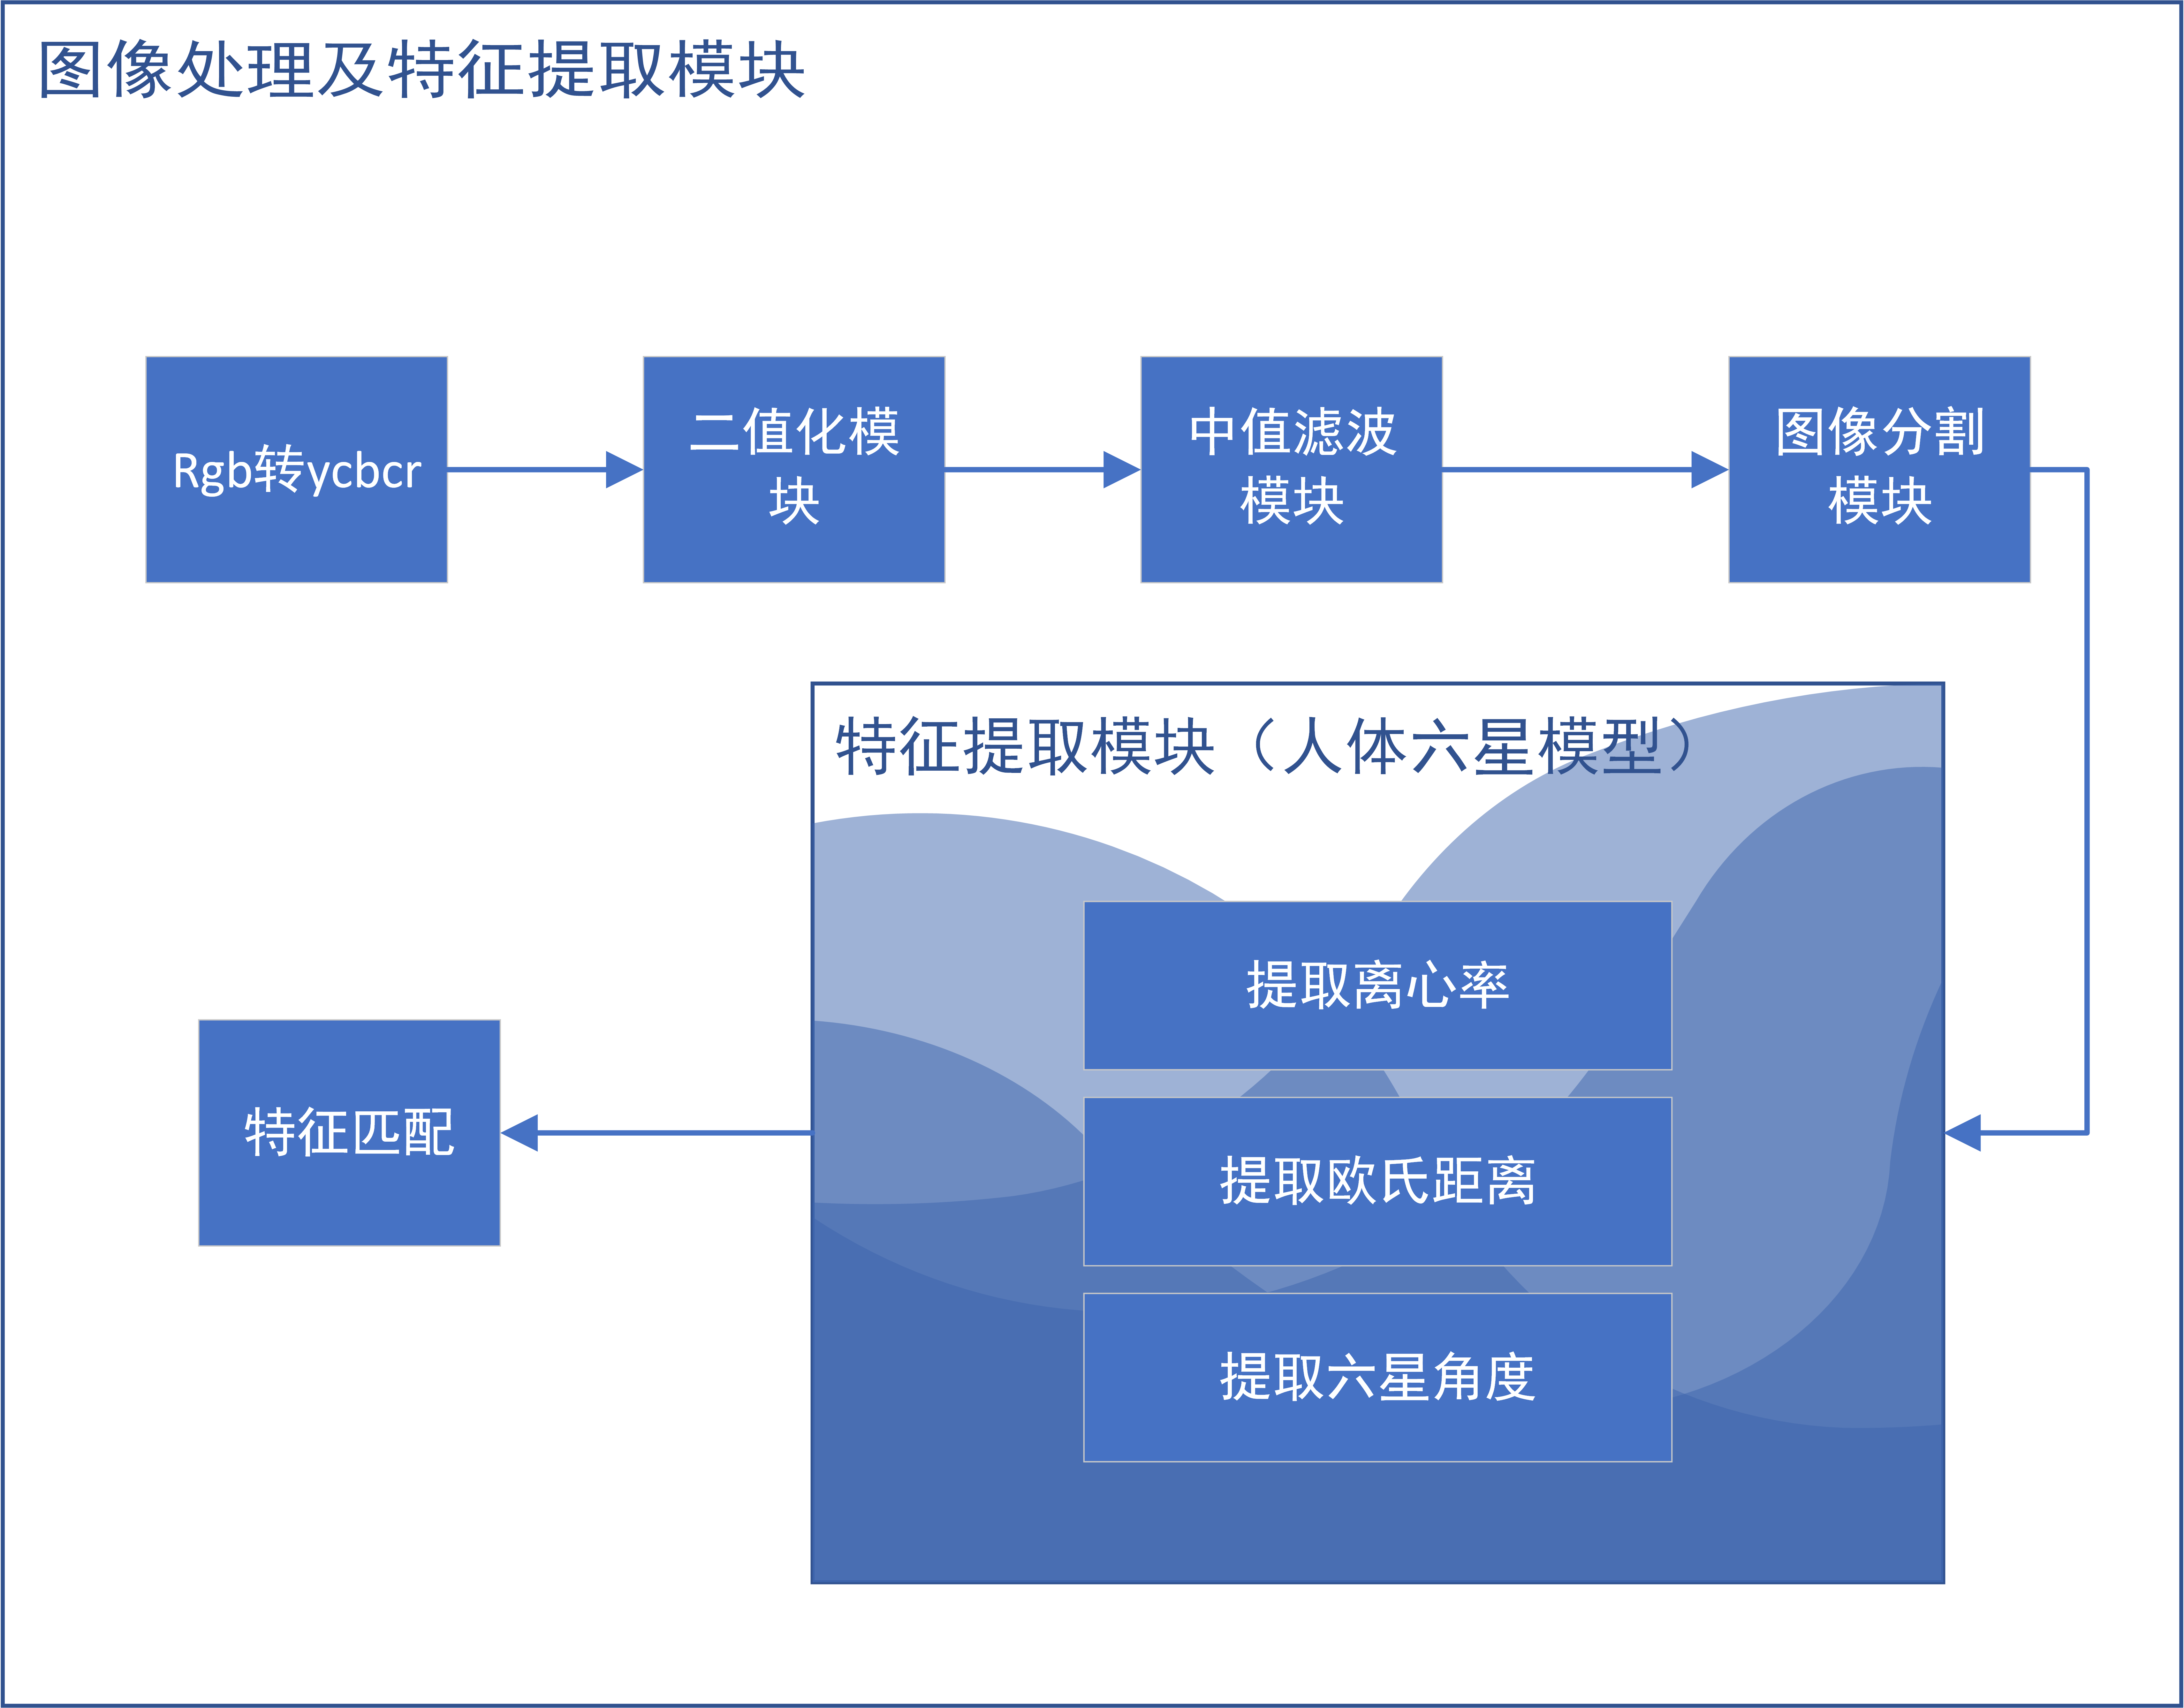
\includegraphics[width=15cm]{figs/f2.png}
    \caption{图像处理和特征提取模块框图}
\end{figure}

其中主要有6个模块。其中rgb转ycbcr模块,二值化模块,中值滤波模块,
图像分割模块对图像作预处理,特征提取模块和特征匹配模块是提取图像的
特征并作匹配,是核心模块。

模块的输入端有帧数据使能信号、帧行同步信号、帧场同步信号、
坐标信号xpos和ypos和像素$pre\_rgb$,这些信号由LCD驱动模块输入。
此模块的输出端除了vip模块处理后的帧数据使能信号、帧行同步信号、
帧场同步信号外,还有一个识别后的数字信号digit。由于达芬奇开发板
板载6位数码管,每位数码管用8421BCD编码显示,总共需要$4\times 6=24$位,
即digit信号位宽为24位,该信号输出给数码管驱动模块在数码管上显
示识别到的数字。

\begin{enumerate}
    \item 图像二值化:在该模块,图像从灰度图像转换为黑白二值图像。
    具体做法为设定一个阈值,判定灰度值高于该阈值即为白色,低于该阈值即为黑色。
    在转换为二值化图像后可以提取出人体的动作,减少背景对姿态识别的干扰,
    便于下一步处理。
    \item 中值滤波:在该模块图像会经过中值滤波处理,得到过滤掉脉冲噪声后的图像。
    中值滤波的原理为用一个检测框固定N*N的范围,并用这N*N个像素点的中值代替该像素
    点中心的灰度值。在本系统中将N设为3。该模块中调用了IP 核 block memory generator
    来完成设计。采用中值滤波可以有效过滤掉背景中和人体附近残余的噪声点,
    从而更有效地识别人体的轮廓和动作。
    \item 投影分割:在该模块会生成一个框住完整图像的最小矩形,确定人体图像的边界。
    模块的工作原理是把图像在水平和垂直方向分别投影,找到黑色像素点的范围,来确定图像的范围。
    \item 特征识别:包括特征提取和特征匹配模块,在特征识别模块会提取出图像的特征
    并与保存在系统中的特征对比,从而识别出该图像是哪种动作。动作识别模块基于人体
    六星模型实现,通过计算人体上6个点和质心的欧氏距离和角度以及最小矩形的离心率
    得到图片的特征向量,通过和标准动作的对比得到最终的识别结果。特征算子提取的流程如
    下图(\ref{f3p})所示,人体六星模型下图(\ref{f4p})所示。

    \begin{figure}[htbp]
        \centering
        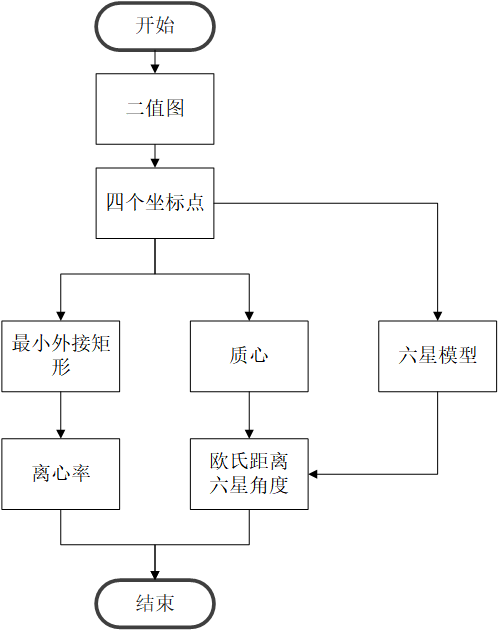
\includegraphics[width=7cm]{figs/f3.png}
        \caption{特征算子提取流程}
        \label{f3p}
    \end{figure}
    \begin{figure}[htbp]
        \centering
        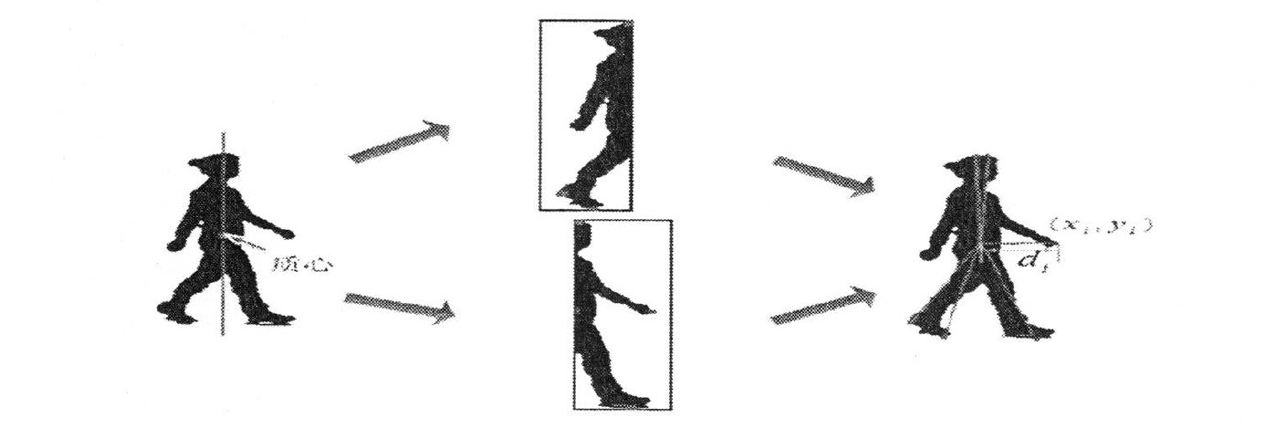
\includegraphics[width=11cm]{figs/f4.png}
        \caption{人体六星模型和质心}
        \label{f4p}
    \end{figure}
    \item 内存模块:该模块的作用是储存经过处理的图像并输出到显示模块。内存模块
    采用了开发板中的DDR3内存(容量为256MB)和IP核FIFO和MIG。
    \item LCD显示模块:LCD模块显示处理之后的图像和找到的最小矩形。
    \item 数码管显示模块:显示识别出的动作编号。

\end{enumerate}

\section{完成情况及性能参数}
如视频所示,通过对摄像头采集到的图像进行预处理并提取特征得到的图像显示在了屏幕上,
同时可见红色的框中为图像处理后图像投影分割的结果。初期,我们共完成了包含5个动作的
动作库的建立。识别后的结果与动作库中的数据比对,匹配结果显示在数码管中。

\begin{figure}[htbp]
    \centering
    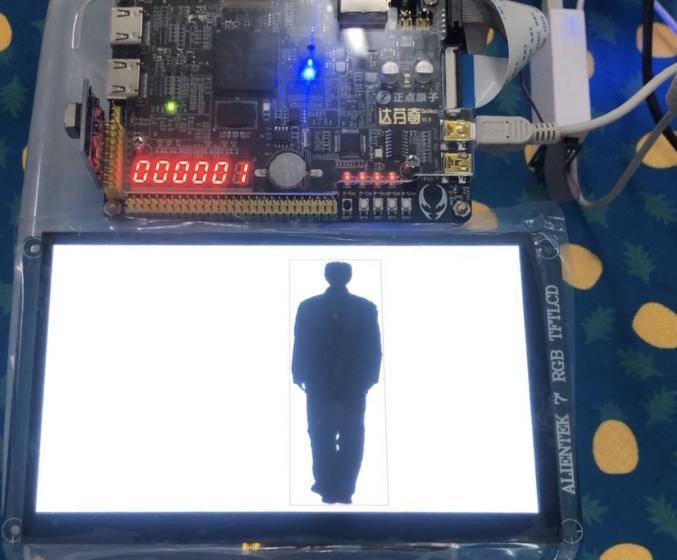
\includegraphics[width=8cm]{figs/f3.jpg}
    \caption{动作1}
\end{figure}
\begin{figure}[htbp]
    \centering
    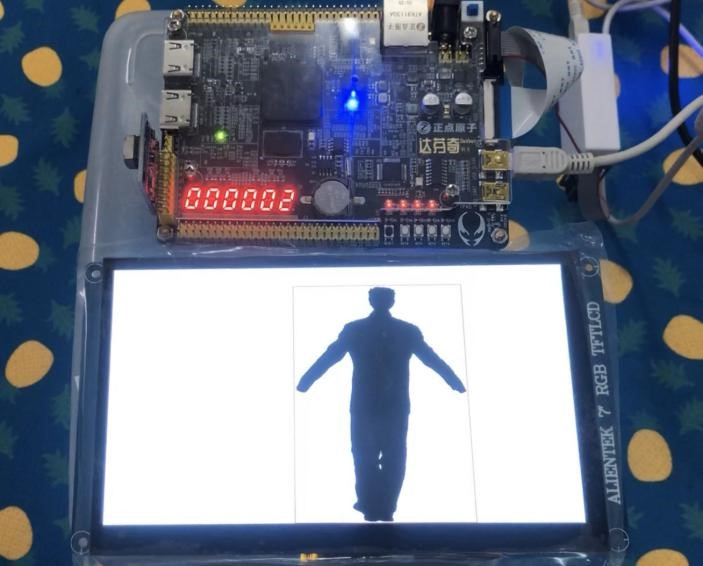
\includegraphics[width=8cm]{figs/f4.jpg}
    \caption{动作2}
\end{figure}
\begin{figure}[htbp]
    \centering
    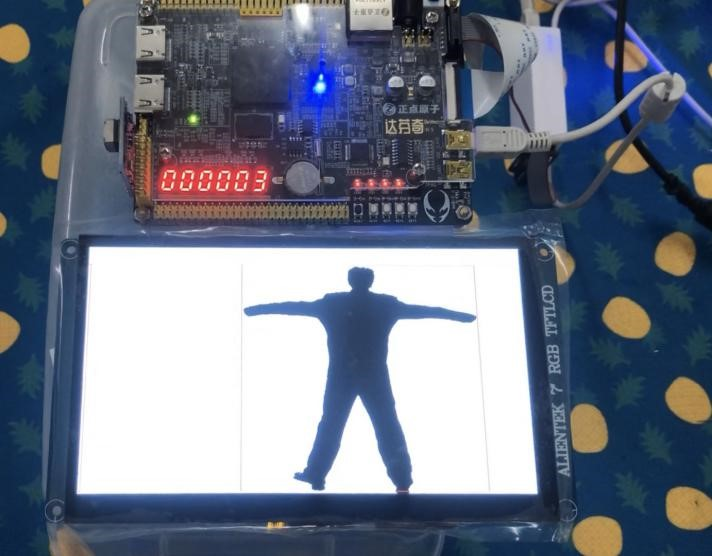
\includegraphics[width=8cm]{figs/f5.jpg}
    \caption{动作3}
\end{figure}
\begin{figure}[htbp]
    \centering
    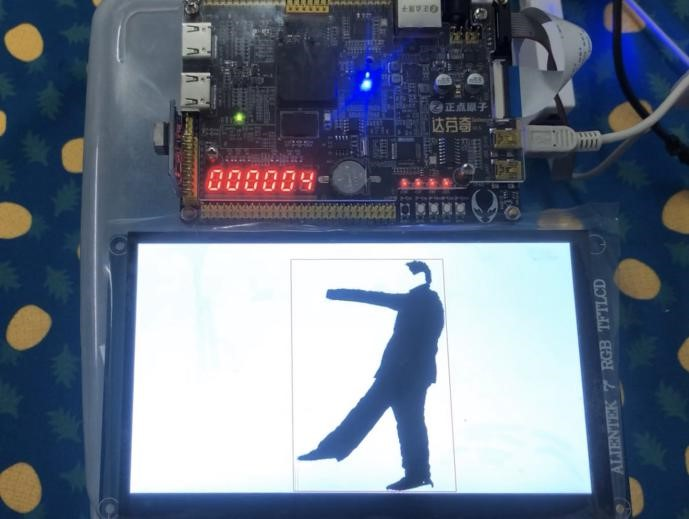
\includegraphics[width=8cm]{figs/f6.jpg}
    \caption{动作4}
\end{figure}
\begin{figure}[htbp]
    \centering
    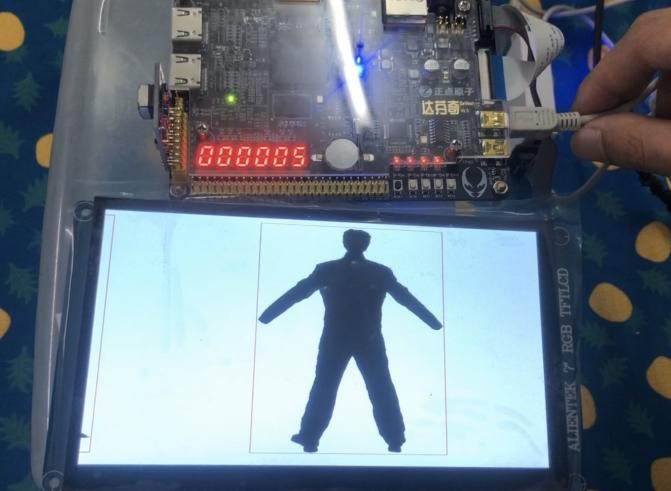
\includegraphics[width=8cm]{figs/f7.jpg}
    \caption{动作5}
\end{figure}
\newpage


\section{总结}
本文基于FPGA对人
体姿态识别系统展开研究,并对每个步骤所采取的方法都做了详细的分析与比
较。从硬件平台的构建,到软件算法的编写,都采取适合于在FPGA平台中实现
的方案,最后实现了一个完整的人体姿态识别系统,并取得了较好的识别效果。
在课题的研究和实现过程中主要完成了以下工作:

本文对姿态识别系统实现的硬件平台、采集设备、
软件算法每一步中的各种方案都进行了实验与比较,最后确定姿态识别系统的实
现方案。

提出性能指标,并在此基础上进行系统的总体设计:然后对组成系统的各个
模块进行实现方案的选取;最后选择合适的硬件平台以及软件开发工具。

根据总体设计阶段得出的结论,进行详细地设计。首先设计系统硬件,选用
Xilinx公司提供的Artix-7开发平台,主要负责姿态图像的预处理和姿态识别
的软件系统的运行。

对姿态识别软件系统的各模块进行设计与实现:使用图像传感器进行图
像采集;使用中值滤波、二值化等方法对图像进行了预处理;根
据人体姿态的七星模型选取13组特征,提取姿态图像的特征参数;最后样本进行分类和姿态识别。

整合系统各个模块,完成系统所要实现的功能。对系统进行综合测试,对测
试结果进行分析,并对系统出现的错误进行改正和调试。

最后,对五种人体姿态进行识别,理想条件下识别率达95\%。


\section{参考文献}
\noindent [1]	唐彪,樊启润,孙开鑫,卢仕,万美琳.人体姿态识别算法在视觉人机交互中的应用[J].计算机测量与控制,2019,27(07):242-247.

\noindent [2]	果彬. 基于FPGA的人体姿态检测与识别系统的设计与实现[D].东北大学,2014.

\noindent [3]	郭天天,杜耀志.基于颜色轮廓的多边形识别及FPGA实现[J].工业控制计算机,2020,33(09):86-88.

\end{document}